\documentclass[11pt]{article}


\usepackage[sort]{natbib}
\usepackage{bm,amsmath,bbm,amsfonts,caption, nicefrac,latexsym,amsmath,amsfonts,amsbsy,amscd,amsxtra,amsgen,amsopn,bbm,amsthm,amssymb,graphicx}
\usepackage{fancyhdr, float}
\usepackage{caption}
\usepackage{subcaption}
\usepackage{color}
\usepackage[margin=1.0in]{geometry}
\usepackage[english]{babel}


\title{Information content for observations of forest carbon stocks and fluxes when assimilated with the DALEC carbon balance model}
%\date{\normalsize{3$^{\text{rd}}$ June 2014, \ Room 1L36}}
\author{\normalsize{E. Pinnington}}


\newtheorem{theorem}{Theorem}[section]
\newtheorem*{defn}{Definition}

	
\begin{document}

\maketitle

\section{Introduction}%%%%%%%%%%%%%%%%%%%%%%

A large amount of data is currently being gathered that is relevant to the carbon balance of forests, with much of this data coming from Eddy covariance flux towers \cite{baldocchi2008turner, baldocchi2001fluxnet, running1999global, valentini2000respiration}. Attempts are also being made to combine this data with models of forest carbon stocks and fluxes, such as the Data Assimilation Linked Ecosystem Carbon model (DALEC), in a data assimilation scheme \cite{williams2005improved, fox2009reflex}. Currently, however, there are limitations with such schemes as there is a lack of understanding about the additional information provided by different observations. Better understanding of the information content of carbon balance observations will help inform measurement campaigns of when and which observations to take, in order to gain the most information possible about the system. In this report, we will look at different information content measures which have been used in meteorological data assimilation \cite{rodgers2000inverse, fisher2003estimation, sandu2012practical} and apply these to carbon balance observations assimilated with DALEC. Although we use DALEC in this report the results will be similar for other carbon balance models which use similar driving data and equations. We begin by introducing the DALEC model which will initially be used to look at the information content in different observations.

\section{The DALEC Model}%%%%%%%%%%%%%%%%%%%%%%

The DALEC model is a simple process-based model describing the carbon balance of an evergreen forest ecosystem \cite{williams2005improved}. The model is constructed of five carbon pools (foliage ($C_f$), fine roots ($C_r$), woody stems and coarse roots ($C_w$), fresh leaf and fine root litter ($C_l$) and soil organic matter and coarse woody debris ($C_s$)) linked via fluxes. The gross primary production function ($GPP$) uses meteorological driving data and the site's leaf area index (a function of $C_f$) to calculate the total amount of carbon to be allocated at a daily time step.   

\begin{figure}[ht]
    \centering
    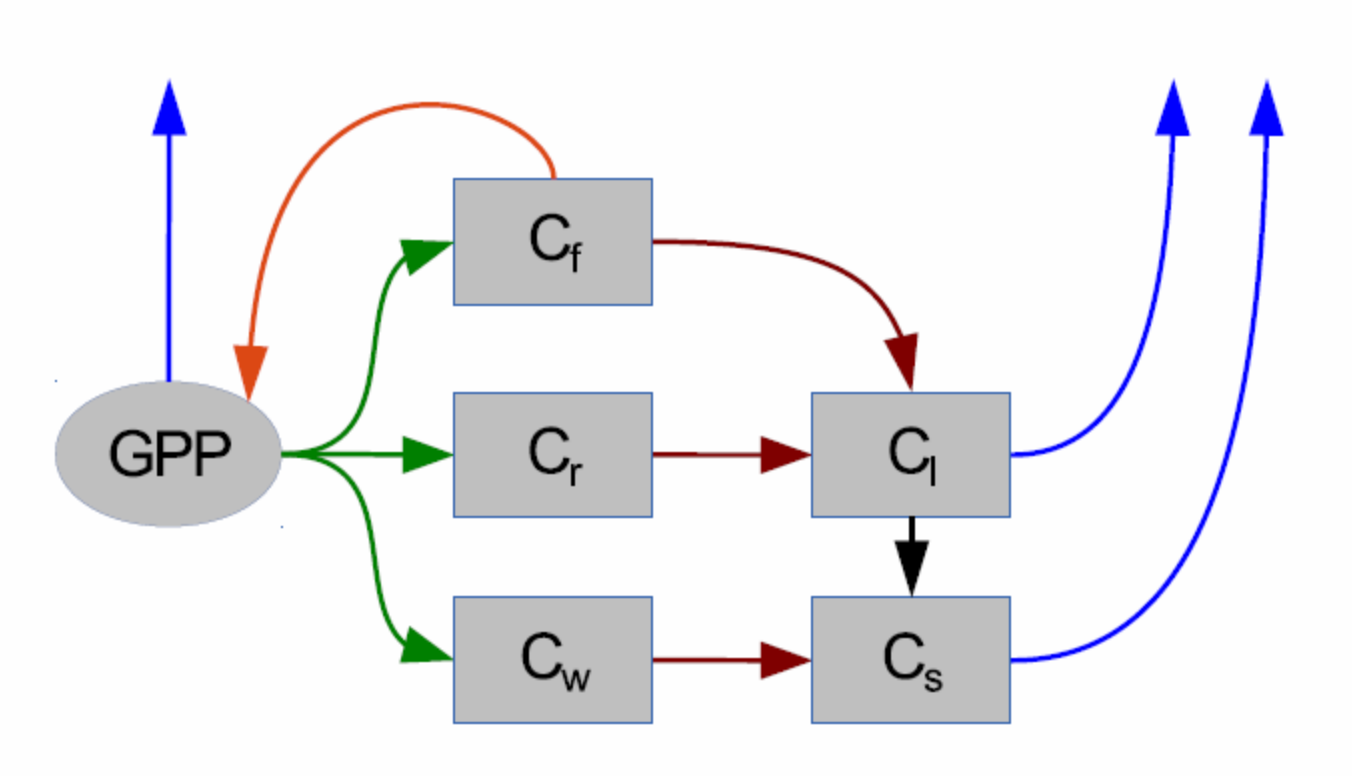
\includegraphics[width=0.5\textwidth]{DALECpic.png}
    \caption{Representation of the carbon fluxes in the DALEC carbon balance model. Green arrows represent C allocation, dark red and black arrows represent litterfall and decomposition fluxes, blue arrows represent respiration fluxes and the light red arrow represents the feedback of foliar carbon to the $GPP$ function. \cite{delahaies2013regularization}}
    \label{fig:DALEC_mod}
\end{figure}

The model equations for the carbon pools at day $t+1$ are as follows:

\begin{align}
C_f(t+1)&=(1-p_5)C_f(t)+p_3(1-p_2)GPP(C_f(t),\phi), \label{dalec1}
\\C_r(t+1)&=(1-p_7)C_r(t)+p_4(1-p_3)(1-p_2)GPP(C_f(t),\phi), 
\\C_w(t+1)&=(1-p_6)C_w(t)+(1-p_4)(1-p_3)(1-p_2)GPP(C_f(t),\phi), 
\\C_l(t+1)&=(1-(p_1+p_8)T(t))C_l(t)+p_5C_f(t)+p_7C_r(t), 
\\C_s(t+1)&=(1-p_9T(t))C_s+p_6C_w(t)+p_1T(t)C_l(t), \label{dalec5}
\end{align}

where $T(t)=\frac{1}{2}exp(p_{10}T_m(t))$, $T_m$ is daily mean temperature, $p_1,\ldots,p_{10}$ are rate parameters and $\phi$ represents the meteorological driving data used in the $GPP$ function. The full details of this version of DALEC can be found in \cite{williams2005improved}. It is parameterized for data from a young pine stand in Ponderossa, Oregon. The model parameters and the equations used to calculate $GPP$ are included in the appendix. We now see how DALEC can be implemented in a four-dimensional variational data assimilation (4D-Var) framework.

\subsection{DALEC in a variational assimilation framework}\label{4dvardalec}%%%%%%%%%%%%%%%%%%%%%% 

In 4D-Var we aim to maximise the probability of our initial state $\textbf{x}_0$ given a set of observations $\textbf{y}$, $P(\textbf{x}_0|\textbf{y})$, over some time window, $N$. For DALEC our state $\textbf{x}_0$ corresponds to the initial values of the five carbon pools,  $\textbf{x}_0 = (C_f(t_0), C_r(t_0), C_w(t_0), C_l(t_0), C_s(t_0))^T$. $P(\textbf{x}_0|\textbf{y})$ is maximised by minimising a cost function $J(\textbf{x})$ derived from Baye's Theorem \cite{lewis2006dynamic}. The cost function is given as,

\begin{equation}
J(\textbf{x}_0) = \frac{1}{2}(\textbf{x}_0-\textbf{x}_b)^{T}\textbf{B}^{-1}(\textbf{x}_0-\textbf{x}_b)+\frac{1}{2}\sum_{i=0}^{N}(\textbf{y}_i-h_i(\textbf{x}_i))^{T}\textbf{R}_{i}^{-1}(\textbf{y}_i-h_i(\textbf{x}_i)),
\end{equation}•
where $\textbf{x}_b$ is our background and acts as our initial guess to our state $\textbf{x}_0$, $\textbf{B}$ is the background error covariance matrix and quantifies our knowledge of the error in our background, $h_i$ is our observation operator at time $t_i$ and maps our state vector evolved by our nonlinear model ($m_{0\rightarrow i}(\mathbf{x}_{0})=\textbf{x}_i$) to the observations at this time $\textbf{y}_i$ and $\textbf{R}_i$ is the observation error covariance matrix and represents our knowledge of the uncertainty in the observations. The state that minimises the cost function is called the analysis and is denoted as $\textbf{x}_a$, this state is found using a minimisation routine that takes the cost function, our initial guess ($\textbf{x}_b$) and also the gradient of the cost function defined as,

\begin{equation}
\nabla J(\textbf{x}_0) = \textbf{B}^{-1}(\textbf{x}_0-\textbf{x}_b)-\sum_{i=0}^{N}\textbf{M}_{i,0}^{T}\textbf{H}_i^{T}\textbf{R}_{i}^{-1}(\textbf{y}_i-h_i(\textbf{x}_i)),
\end{equation}•
where $\textbf{H}_i = \frac{\delta h_i(\textbf{x}_i)}{\delta\textbf{x}_i}$ is our linearized observation operator and $\mathbf{M}_{i,0}=\mathbf{M}_{i-1}\mathbf{M}_{i-2}\cdots\mathbf{M}_0$ is our tangent linear model with $\mathbf{M}_i=\frac{\delta m_{i}(\textbf{x}_{i})}{\delta \textbf{x}_{i}}$. We can calculate the linearized model for DALEC from equations \ref{dalec1} to \ref{dalec5} as,
\begin{equation}
\mathbf{M}_{i}= 
\begin{pmatrix} 
(1-p_5)+p_3(1-p_2)\zeta_i & 0 & 0 & 0 & 0 \\
p_4(1-p_3)(1-p_2)\zeta_i & (1-p_7) & 0 & 0 & 0 \\
(1-p_4)(1-p_3)(1-p_2)\zeta_i & 0 & (1-p_6) & 0 & 0 \\
p_5 & p_7 & 0 & (1-(p_1+p_8)T_i) & 0 \\
0 & 0 & p_6 & p_1T_i & (1-p_9T_i) \\
\end{pmatrix}, \label{linmod}
\end{equation}
where $\zeta_i = GPP'(C_f(t_i), \phi)$ and $T_{i}=T(t_i)$. In 4D-Var we assume the tangent linear hypothesis,
\begin{equation}
m_{0\rightarrow i}(\mathbf{x}_0+\delta\mathbf{x}_0) \approx m_{0 \rightarrow i}(\mathbf{x}_0) + \mathbf{M}_{i,0}\delta\mathbf{x}_0. \label{TLH}
\end{equation}•
The validity of this assumption depends on how nonlinear the model is, the length of the assimilation window and the size of the perturbation $\delta\mathbf{x}_0$. We can test the validity for DALEC by taking our initial states from the appendix for $\mathbf{x}_0$ and a $5\%$ perturbation for $\delta\mathbf{x}_0$. We then rearrange equation \ref{TLH} to find, 
\begin{equation}
\text{Percentage error in tangent linear model} = \begin{vmatrix} \frac{m_{0\rightarrow i}(\mathbf{x}_0+\delta\mathbf{x}_0) - m_{0 \rightarrow i}(\mathbf{x}_0)}{ \mathbf{M}_{i,0}\delta\mathbf{x}_0} - 1 \end{vmatrix} \times 100.
\end{equation}• 
The percentage error in our approximation at each time step for each carbon pool when the model is run forward for 1000 days is shown in figure \ref{linerr}.
\begin{figure}[H]
\centering
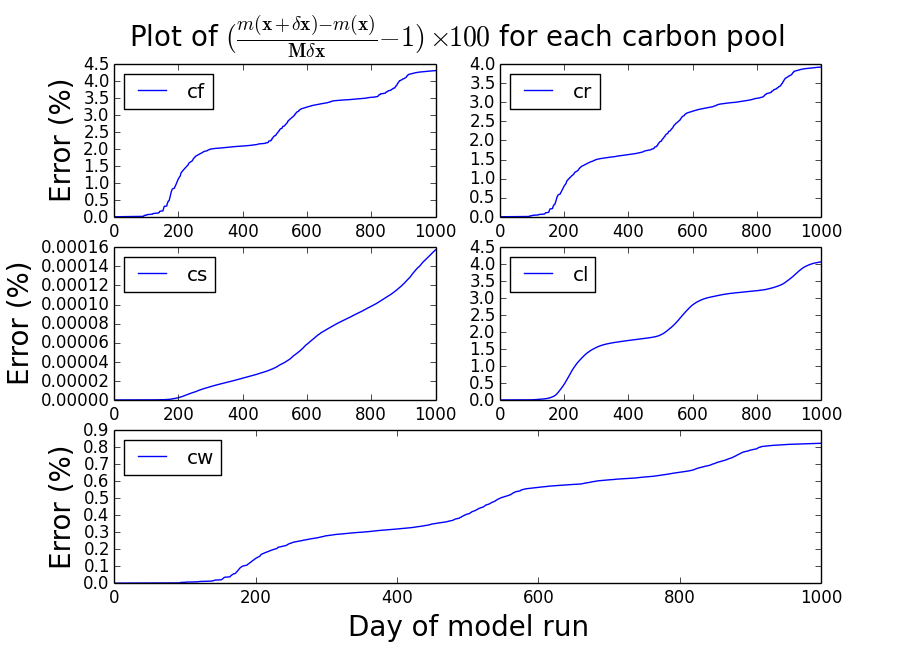
\includegraphics[height=.4\textwidth]{Sub_linerr.png}
\caption{Percentage error in linear model for each carbon pool when run forward for 1000 days.}
\label{linerr}
\end{figure}
We see that the error grows as we get further away from the start of our run. We also see that the carbon pools with the most error ($C_f$, $C_r$ and $C_l$) are the ones most dependent on $GPP$, the only nonlinear term in our model. Figure \ref{linerr} shows us that for DALEC the tangent linear hypothesis is not a bad approximation.

Once we have performed the minimisation of the cost function and determined $\textbf{x}_a$, we can also calculate the analysis error covariance matrix, $\textbf{A}$, to quantify the uncertainty in our new estimate of the state. We define the analysis error covariance matrix as,
\begin{equation}
\textbf{A} = \big(\mathbf{J}''\big)^{-1} = \big(\mathbf{B}^{-1}+\hat{\mathbf{H}}^{T}\hat{\mathbf{R}}^{-1}\hat{\textbf{H}}\big)^{-1}, \label{Amat}
\end{equation}• 
where $\hat{\mathbf{H}}$ is the matrix of linearized observation operators evolved by the tangent linear model and $\hat{\mathbf{R}}$ is the block diagonal matrix of observation error covariance matrices,
\begin{equation}
\hat{\mathbf{H}}=
\begin{pmatrix}
\mathbf{H}_0 \\
\mathbf{H}_1\mathbf{M}_0\\
\vdots \\
\mathbf{H}_N\mathbf{M}_{N,0}
\end{pmatrix}
\hspace{5mm} \text{and} \hspace{5mm}
\hat{\mathbf{R}}=
\begin{pmatrix}
\mathbf{R}_0 & 0 & 0 & 0 \\
0 & \mathbf{R}_1 & 0 & 0 \\
0 & 0 & \ddots & 0 \\
0 & 0 & 0 & \mathbf{R}_N
\end{pmatrix}.
\end{equation}
It is important to note that we do not need any actual observations to calculate $\textbf{A}$, $\textbf{J}''$ or $\textbf{B}$, only the values of the standard deviations for the observations and the standard deviations for our background values.  

\section{Information Content Measures}%%%%%%%%%%%%%%%%%%%%%%

Information content measures are already being used to quantify the different levels of information provided by observations in the development of satellite instruments \cite{stewart2008correlated, engelen2004information} and in operational data assimilation schemes \cite{fisher2003estimation, sandu2012practical}. In these fields, two of the more widely used measures are Shannon Information Content (also known as entropy reduction) and the degrees of freedom for signal. We will apply both methods for observations assimilated with DALEC. 

\subsection{Shannon Information Content}%%%%%%%%%%%%%%%%%%%%%%

In DA, Shannon Information Content ($SIC$) is a measure of the reduction in entropy given a set of observations. Entropy physically corresponds to the volume in state space taken up by the probability density function ($pdf$) describing the knowledge of the state. When a measurement is made, the volume of this $pdf$ decreases. The $SIC$ of the measurement is a measure of the factor by which the $pdf$ decreases \cite{rodgers2000inverse}. If $P_b(x)$ is our knowledge of the state before an observation and $P_o(x|y)$ is our knowledge after an observation then we have entropies,
\[
S[P_b(x)] = - \int P_b(x)\text{log}_2[P_b(x)]dx
 \hspace{5mm} \text{and} \hspace{5mm} 
S[P_o(x|y)] = - \int P_o(x|y)\text{log}_2[P_o(x|y)]dx.
\]
The entropy reduction, or $SIC$, due to the observation is then,
\begin{equation} \label{shaic}
SIC =  S[P_b(x)]-S[P_o(x|y)].
\end{equation}
If we assume all $pdfs$ are Gaussian and use the natural logarithm as opposed to $\text{log}_2$ (for algebraic convenience) \cite{rodgers2000inverse}, the entropy of a multivariate Gaussian distruibution for a vector $\textbf{x}$ with $n$ elements (before and after observations) can be derived as,
\begin{equation} \label{SB}
 S[P_b(\textbf{x})] = n\text{ln}(2\pi e)^{\frac{1}{2}}+\frac{1}{2}\text{ln}\begin{vmatrix}\bf{B}\end{vmatrix}
\end{equation}
and
\begin{equation} \label{SA}
 S[P_o(\textbf{x}|\textbf{y})] = n\text{ln}(2\pi e)^{\frac{1}{2}}+\frac{1}{2}\text{ln}\begin{vmatrix}\bf{A}\end{vmatrix}
\end{equation}
where $\bf{B}$ is the background error covariance matrix and $\bf{A}$ is the analysis error covariance matrix. Combining equations \ref{shaic}, \ref{SB} and \ref{SA} we can write the $SIC$ as,
\begin{equation}
SIC=\frac{1}{2}\text{ln}\frac{\begin{vmatrix} \bf{B} \end{vmatrix}}{\begin{vmatrix} \bf{A} \end{vmatrix}}.
\end{equation}•
From equation \ref{Amat} we can see the $SIC$ can also be written as,
\begin{equation}
SIC= \frac{1}{2}\text{ln}\begin{vmatrix} \mathbf{B} \end{vmatrix}\begin{vmatrix} \mathbf{J}'' \end{vmatrix}. \label{sic}
\end{equation}•

\subsection{Degrees of Freedom for Signal} \label{DFSintro}%%%%%%%%%%%%%%%%%%%%%%

The degrees of freedom for signal ($DFS$) indicates the number of elements of the state that have been measured by the observations. If we consider a state vector $\textbf{x}$ with $n$ elements (or $n$ degrees of freedom) then the maximum value the $DFS$ could obtain would be $n$, in this case all elements of the state would have been measured. Conversely if $DFS = 0$ then no elements of the state would have been measured by our observations \cite{fowler2011measures}.

We have symmetric positive definite background and analysis error covariance matrices $\bf{B}$ and $\bf{A}$. The eigenvalues of each matrix gives a representation for the uncertainty in the direction of the associated eigenvector, thus, by comparing the eigenvalues of both matrices we can determine the reduction in uncertainty given a set of observations \cite{stewart2008correlated}.

In order to do this we take $\mathbf{B}^{\frac{-1}{2}}$ such that $\mathbf{B}^{-1} = \mathbf{B}^{\frac{-1}{2}}\mathbf{B}^{\frac{-1}{2}}$. We now take $\bf{Q}$ to be the orthogonal matrix composed of the eigenvectors of $\mathbf{B}^{\frac{-1}{2}}\mathbf{A}\mathbf{B}^{\frac{-1}{2}}$ we have,
\begin{equation}
\mathbf{Q}^{T}\bigg(\mathbf{B}^{\frac{-1}{2}}\mathbf{A}\mathbf{B}^{\frac{-1}{2}}\bigg)\mathbf{Q} = \bf{\Lambda},
\end{equation}• 
\begin{equation}
\mathbf{Q}^{T}\bigg(\mathbf{B}^{\frac{-1}{2}}\mathbf{B}\mathbf{B}^{\frac{-1}{2}}\bigg)\mathbf{Q} = \mathbf{I}_{n\times n}
\end{equation}•
where $\bf{\Lambda}$ is a diagonal matrix. Each diagonal element of our transformed $\bf{B}$ is equal to one and corresponds to one degree of freedom. The diagonal elements of $\bf{\Lambda}$ correspond to the matrix's eigenvalues and can be interpreted as the relative reduction in variance for each of the $n$ degrees of freedom \cite{sandu2012practical}. We can then define the $DFS$ as,
\begin{equation}
\begin{split}
DFS & = \text{trace}(\mathbf{I}_{n\times n} - \mathbf{\Lambda}) \\
       & = n - \text{trace}(\mathbf{\Lambda}) \\
       & = n - \text{trace}(\mathbf{B}^{\frac{-1}{2}}\mathbf{A}\mathbf{B}^{\frac{-1}{2}}) \\
       & = n - \text{trace}(\mathbf{B}^{-1}\mathbf{A}).
\end{split}
\end{equation}

\section{Shannon Information Content for DALEC}%%%%%%%%%%%%%%%%%%%%%%

We begin by using $SIC$ to understand the information content for different observations when being assimilated with the DALEC model. For these experiments the model is set up as in section \ref{4dvardalec} where the elements of the state vector have standard deviations, $\sigma_{cf,b},\ldots,\sigma_{cs,b}$, respectively. These standard deviations represent the uncertainty in our inital background estimate, and are taken as a percentage of the initial carbon pools (these values can be found in the appendix). The background error covariance matrix is then taken as the diagonal matrix of the variances of the carbon pools,
\begin{equation}
\bf{B} = \begin{pmatrix} 
\sigma_{cf,b}^{2} & 0 & 0 & 0 & 0 \\
0 & \sigma_{cr,b}^{2} & 0 & 0 & 0 \\
0 & 0 & \sigma_{cw,b}^{2} & 0 & 0 \\
0 & 0 & 0 & \sigma_{cl,b}^{2} & 0 \\
0 & 0 & 0 & 0 & \sigma_{cs,b}^{2} \\
\end{pmatrix}. \label{Bmat}
\end{equation}

Our initial experiments look at the $SIC$ in observations taken at a single time; the 4D-Var data assimilation then becomes three-dimensional variational assimilation (3D-Var) as we are not summing over a time window and have no time component.

\subsection{$SIC$ for a single observation at one time} \label{sic1time}%%%%%%%%%%%%%%%%%%%%%%

If we first consider one observation of $C_f$ (the first element of our state vector $\textbf{x}$) at time $t_0$, we can derive an analytical expression for the $SIC$ using,
\begin{equation}
\mathbf{H}_{0} = \frac{\delta C_f(t_0)}{\delta\textbf{x}_0} = \begin{pmatrix}
1 & 0 & 0 & 0 & 0
\end{pmatrix},
\end{equation} 
where $\mathbf{H}_{0}$ is our linearized observation operator at time $t_0$. As we have a single observation at one time, our observation error covariance matrix, $\bf{R}_0$, is just the variance of our observation of $C_f$ at time $t_0$ ($\sigma_{cf,o}^{2}$). Therefore,
\begin{equation}
\mathbf{R}_0=\sigma_{cf,o}^{2}.
\end{equation}
We then have from equation \ref{Amat},
\begin{equation}
\begin{array} {lcl}
\mathbf{J}'' &=& \mathbf{B}^{-1}+\hat{\mathbf{H}}^{T}\hat{\mathbf{R}}^{-1}\hat{\mathbf{H}} \\
&=& \mathbf{B}^{-1}+\mathbf{H}_0^{T}\mathbf{R}_0^{-1}\mathbf{H}_0 \\
&=& \begin{pmatrix} 
\sigma_{cf,b}^{-2}+\sigma_{cf,o}^{-2} & 0 & 0 & 0 & 0 \\
0 & \sigma_{cr,b}^{-2} & 0 & 0 & 0 \\
0 & 0 & \sigma_{cw,b}^{-2} & 0 & 0 \\
0 & 0 & 0 & \sigma_{cl,b}^{-2} & 0 \\
0 & 0 & 0 & 0 & \sigma_{cs,b}^{-2} \\
\end{pmatrix}.
\end{array}
\end{equation} 
We can now derive the $SIC$ using equation \ref{sic} as,
\begin{equation}
SIC = \frac{1}{2}\text{ln}\begin{vmatrix} \mathbf{B} \end{vmatrix}\begin{vmatrix} \mathbf{J}'' \end{vmatrix}= \frac{1}{2}\text{ln}\frac{(\sigma_{cf,o}^{2}+\sigma_{cf,b}^{2})}{\sigma_{cf,o}^{2}}
=\frac{1}{2}\text{ln} \bigg(1+\frac{\sigma_{cf,b}^{2}}{\sigma_{cf,o}^{2}}\bigg). \label{siccf1time}
\end{equation}
We see the $SIC$ for an observation of a single observation of $C_f$ is dependent on the ratio between the observation and background variances; the $SIC$ will have the same form for all other direct observations of carbon pools contained in the state. As our background standard deviations are set to being the same percentage for each carbon pool (see appendix), the carbon pool observation which will give us the highest $SIC$ is the pool that we can measure most accurately as this will maximise the ratio $\frac{\sigma_{c,b}^{2}}{\sigma_{c,o}^{2}}$ by minimising $\sigma_{c,o}^{2}$.

One of the main carbon balance observations made at forest flux tower sites is the net ecosystem exchange ($NEE$) of CO$_{2}$, which can be estimated by DALEC as the difference between $GPP$ and the respirations of $C_l$ and $C_s$, giving,
\begin{equation}
NEE(t)=-(1-p_2)GPP(C_f(t),\phi)+p_8C_lT(t)+p_9C_sT(t). \label{neeeqn}
\end{equation}
For a single observation of $NEE$ at one time, $t_0$, we can again derive an analytical expression for the $SIC$ using,
\begin{equation}
\mathbf{H}_{0}=\frac{\delta NEE(t_0)}{\delta\textbf{x}_0} = \begin{pmatrix}
-(1-p_{2})\zeta_0 & 0 & 0 & p_{8}T_{0} & p_{9}T_{0}
\end{pmatrix},
\end{equation}
where $\zeta_0 = GPP'(C_f(t_0), \phi)$, $T_{0}=T(t_0)$ and $\mathbf{H}_{0}$ is the linearized observation operator at time $t_0$. Again our observation error covariance matrix, $\bf{R}_0$, is just the variance of our observation of $NEE$, $\sigma_{nee,o}^{2}$, at time $t_0$. Therefore,
\begin{equation}
\mathbf{R}_0=\sigma_{nee,o}^{2}
\end{equation}
and again,
\begin{equation}
\begin{array} {lcl}
\mathbf{J}'' &=& \mathbf{B}^{-1}+\mathbf{H}_0^{T}\mathbf{R}_0^{-1}\mathbf{H}_0 \\
&=& \begin{pmatrix} 
\sigma_{cf,b}^{-2}+\sigma_{nee,o}^{-2}(1-p_{2})^{2}\zeta_0^{2} & 0 & 0 & \sigma_{nee,o}^{-2}(1-p_{2})\zeta_0 p_{8}T_0 & \sigma_{nee,o}^{-2}(1-p_{2})\zeta_0 p_{9}T_0 \\
0 & \sigma_{cr,b}^{-2} & 0 & 0 & 0 \\
0 & 0 & \sigma_{cw,b}^{-2} & 0 & 0 \\
\sigma_{nee,o}^{-2}(1-p_{2})\zeta_0 p_{8}T_0 & 0 & 0 & \sigma_{cl,b}^{-2}+\sigma_{nee,o}^{-2}p_{8}^2 T_0^2 & \sigma_{nee,o}^{-2}p_{8}p_{9} T_0^2 \\
\sigma_{nee,o}^{-2}(1-p_{2})\zeta_0 p_{9}T_0 & 0 & 0 & \sigma_{nee,o}^{-2}p_{8}p_{9} T_0^2 & \sigma_{cs,b}^{-2}+\sigma_{nee,o}^{-2}p_{9}^2 T_0^2 \\
\end{pmatrix}.
\end{array}
\end{equation} 
We then have,
\begin{equation}
SIC = \frac{1}{2}\text{ln}\begin{vmatrix} \mathbf{B} \end{vmatrix}\begin{vmatrix} \mathbf{J}'' \end{vmatrix} = \frac{1}{2}\text{ln}\frac{(p_{2}-1)^{2}\zeta_0^{2}\sigma_{cf,b}^{2}+\sigma_{nee,o}^{2}+T_{0}^2(p_{9}^2\sigma_{cs,b}^2+p_8^2\sigma_{cl,b}^2)}{\sigma_{nee,o}^{2}}.
\end{equation}

If we assume that the variances and parameters here are fixed, we can see that the size of the $SIC$ is dependent on the temperature term, $T_0$, and the square of the first derivative of $GPP$, $\zeta_0^{2}$. Generally, the value of $GPP$ (and its first derivative) is highest in summer with higher temperatures and higher total daily irradiance. We therefore have that there will be more information content in observations that are taken when temperatures are higher. Physically this makes sense as more $NEE$ takes place when temperatures are higher (to a point), so measurements are of greater magnitude and give us more information about carbon fluxes. 

By plotting the $SIC$ for a single observation of $NEE$, varying with three years of meteorological driving data, next to the temperature term ($T(t_i)$) for the same data we can see that both are closely linked, figure \ref{fig:SICNEET}.
\begin{figure}[H]
\centering
\begin{subfigure}{.5\textwidth}
  \centering
  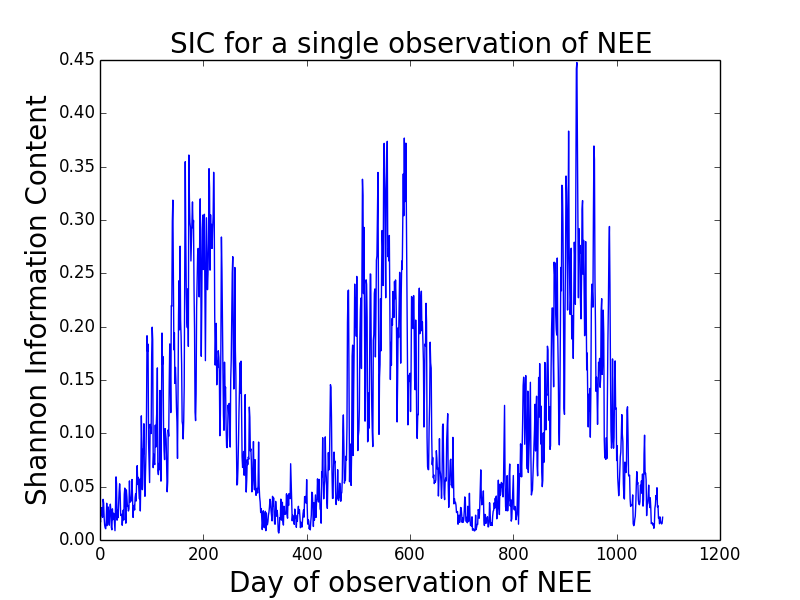
\includegraphics[width=.9\linewidth]{SIC1Obs_0_1095.png}
  \caption{$SIC$ for a single observation of $NEE$.}
  \label{fig:sub1}
\end{subfigure}%
\begin{subfigure}{.5\textwidth}
  \centering
  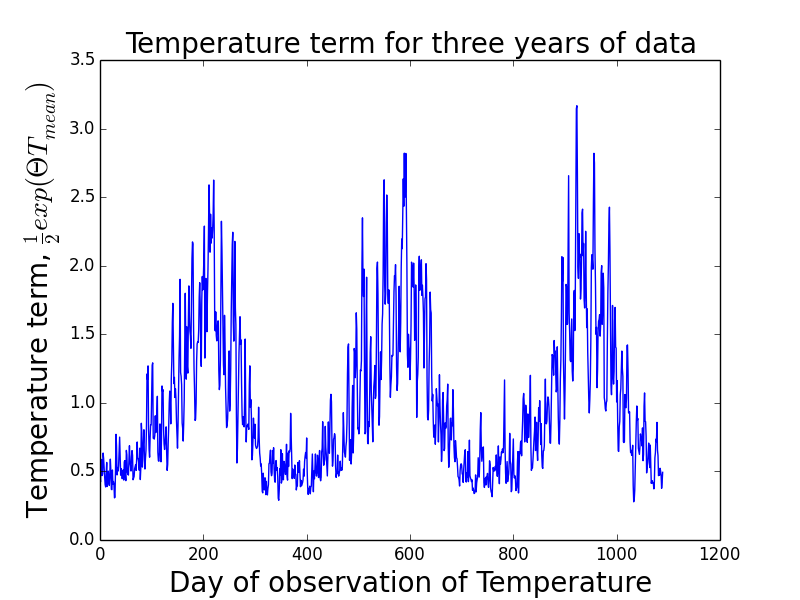
\includegraphics[width=.9\linewidth]{Temp_0_1095.png}
  \caption{Temperature term, $\frac{1}{2}exp(\Theta  T_{mean})$.}
  \label{fig:sub2}
\end{subfigure}
\caption{$SIC$ and temperature varying over three years using driving data from Oregon pine forest.}
\label{fig:SICNEET}
\end{figure}
However the relationship is not linear as the magnitude of $GPP$'s first derivative is also dependent on daily irradiance and the value of the foliar carbon pool ($C_f$). This shows that observations of $NEE$ made in the summer are much more valuable than those made in the winter assuming warmer temperatures, higher daily irradiance and a higher amount of foliar carbon in the summer. In the next section we consider a series of observations over some time window. We will see that it takes up to 31 observations of $NEE$ in winter to gain the same level of information as 1 observation of $NEE$ in the summer.

\subsection{$SIC$ for successive observations over a time window} \label{SICsucc}%%%%%%%%%%%%%%%%%%%%%%

Following the results for $SIC$ based at a single time, we now consider the $SIC$ when successive observations are added over a period of time. We begin by considering two successive observations of $Cf$ in time. From section \ref{4dvardalec} and \ref{sic1time} we have our linearized observation operator and observation error covariance matrix at time $t_i$,
\begin{equation}
\mathbf{H}_{i} = \frac{\delta C_f(t_i)}{\delta\textbf{x}_i} = \begin{pmatrix}
1 & 0 & 0 & 0 & 0
\end{pmatrix}
\hspace{5mm} \text{and} \hspace{5mm}
\mathbf{R}_i=\sigma_{cf,o}^{2}.
\end{equation}
Then for two successive observations of $Cf$ we have,
\begin{equation}
\hat{\mathbf{H}}=
\begin{pmatrix}
\mathbf{H}_0 \\
\mathbf{H}_1\mathbf{M}_0\\
\end{pmatrix}
=
\begin{pmatrix}
1 & 0 & 0 & 0 & 0 \\
(1-p_5)+p_3(1-p_2)GPP'(C_f(t_0),\phi) & 0 & 0 & 0 & 0\\
\end{pmatrix}
\end{equation}
and
\begin{equation}
\hat{\mathbf{R}}=
\begin{pmatrix}
\mathbf{R}_0 & 0  \\
0 & \mathbf{R}_1  \\
\end{pmatrix}
=
\begin{pmatrix}
\sigma_{cf,o}^{2} & 0  \\
0 & \sigma_{cf,o}^{2}  \\
\end{pmatrix}.
\end{equation}
We then have,
\begin{equation}
SIC = \frac{1}{2}\text{ln}\begin{vmatrix} \mathbf{B} \end{vmatrix}\begin{vmatrix} \mathbf{J}'' \end{vmatrix} =\frac{1}{2}\text{ln} \bigg(1+\frac{\sigma_{cf,b}^{2}}{\sigma_{cf,o}^{2}}+\frac{\sigma_{cf,b}^{2}\eta_0^{2}}{\sigma_{cf,o}^{2}} \bigg),
\end{equation}
where $\eta_i=(1-p_5)+p_3(1-p_2)GPP'(C_f(t_i),\phi)$. We see this is similar to equation \ref{siccf1time} but with an extra term, $\eta_0^2$, which is the square of the first element of our linearized model $\mathbf{M}_0$. We can continue adding more observations at successive times and we start to see a pattern. For three observations at successive times we have,
\begin{equation}
SIC =\frac{1}{2}\text{ln} \bigg(1+\frac{\sigma_{cf,b}^{2}}{\sigma_{cf,o}^{2}}+\frac{\sigma_{cf,b}^{2}\eta_0^{2}}{\sigma_{cf,o}^{2}}+\frac{\sigma_{cf,b}^{2}\eta_0^{2}\eta_1^{2}}{\sigma_{cf,o}^{2}} \bigg),
\end{equation}
for four,
\begin{equation}
SIC =\frac{1}{2}\text{ln} \bigg(1+\frac{\sigma_{cf,b}^{2}}{\sigma_{cf,o}^{2}}+\frac{\sigma_{cf,b}^{2}\eta_0^{2}}{\sigma_{cf,o}^{2}}+\frac{\sigma_{cf,b}^{2}\eta_0^{2}\eta_1^{2}}{\sigma_{cf,o}^{2}}+\frac{\sigma_{cf,b}^{2}\eta_0^{2}\eta_1^{2}\eta_2^{2}}{\sigma_{cf,o}^{2}} \bigg).
\end{equation}
Using a simple proof by induction we find that for $n$ observations we have,
\begin{equation}
SIC\text{ for }n\text{ observations of }C_f = \frac{1}{2}\text{ln}\bigg(1+\frac{\sigma_{cf,b}^{2}}{\sigma_{cf,o}^{2}}\big(1+\sum_{k=0}^{n-2}\prod_{i=0}^{k}\eta_i^{2}\big)\bigg).
\end{equation}
We have plotted the $SIC$ for increasing numbers of observations of $C_f$, using three years of meteorological driving data from the Oregan pine forest, as seen in figure \ref{Cf_succ}.

\begin{figure}[H]
\centering
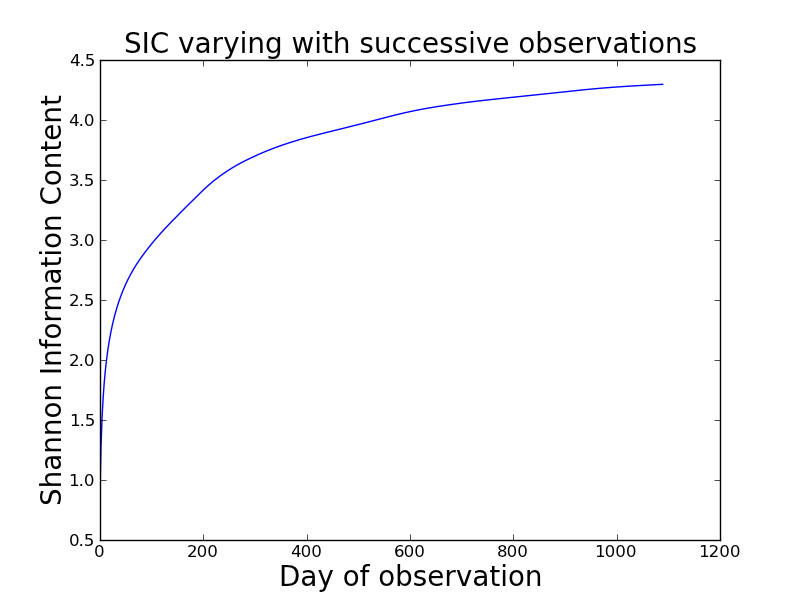
\includegraphics[height=.34\textwidth]{SIC0_1090cf.png}
\caption{$SIC$ varying as successive observations of $Cf$ are added using driving data from Oregon pine forest.}
\label{Cf_succ}
\end{figure}

We can see after around 250 observations of $C_f$ have been made, our $SIC$ starts to level off as we are getting a smaller and smaller reduction in entropy for the extra observations of $C_f$ being made. We see this effect when making successive observations of any of the carbon pools, eventually we cannot reduce the entropy of the system anymore by just adding more of the same observation.  

As before with a single observation at one time we can repeat this with successive observations of $NEE$ instead of $C_f$, this is plotted in figure \ref{SIC_succ}. Here we see a similar levelling off in $SIC$ as in figure \ref{Cf_succ}, we can also see the seasonal cycle of information content in $NEE$ as in figure \ref{fig:SICNEET}. Once the $SIC$ has levelled off no information is added during the winter months and the $SIC$ is only increased with observations made during the summer.

\begin{figure}[H]
\centering
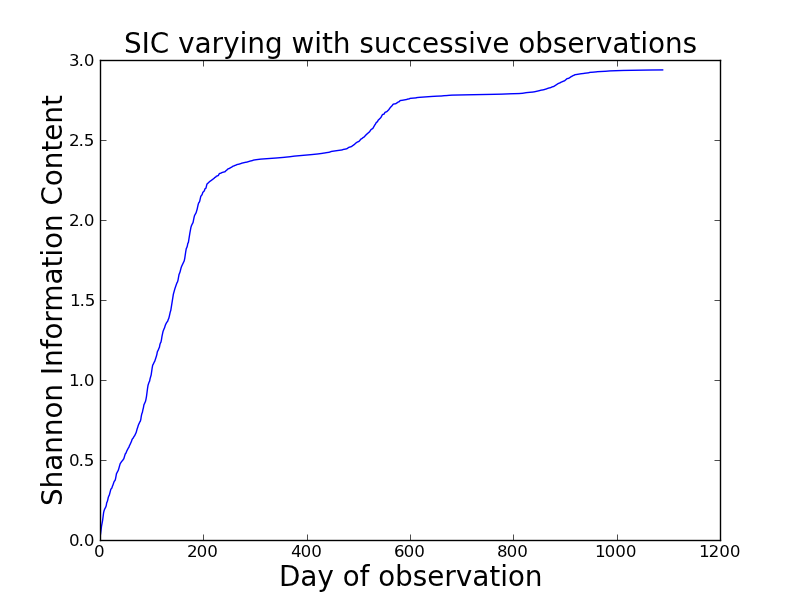
\includegraphics[height=.34\textwidth]{SIC0_1090nee.png}
\caption{$SIC$ varying as successive observations of $NEE$ are added using driving data from Oregon pine forest.}
\label{SIC_succ}
\end{figure} 

We can also repeat this with successive observations of both $NEE$ and $C_f$, this can be seen in figure \ref{fig:SIC_neecfsubplot}. We attain a higher value of $SIC$ more quickly than before and reach a higher overall value of $SIC$ than in figure \ref{SIC_succ} or \ref{Cf_succ}. We reduce the entropy of our system very little when adding extra observations of $C_f$ and $NEE$ by day 600.

\begin{figure}[H]
\centering
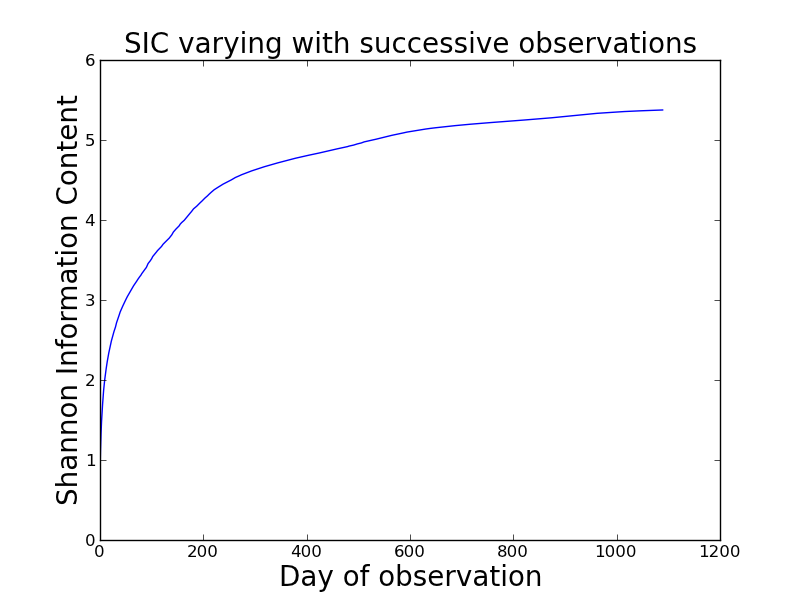
\includegraphics[height=.34\textwidth]{SIC0_1090cfnee.png}
\caption{$SIC$ varying as successive observations of $NEE$ and $Cf$ are added using driving data from Oregon pine forest.}
\label{fig:SIC_neecfsubplot}
\end{figure}

In order to see the difference in information content between $NEE$ observations made in the summer and those made in the winter, we have plotted the increasing $SIC$ for 50 observations made from December $21^{\text{st}}$ onwards and also the the constant line of $SIC$ for one observation of $NEE$ made in summer at a mean daily temperature of $26^{o}\text{C}$ on July $12^{\text{th}}$. This is shown in figure \ref{summwintsic}

\begin{figure}[H]
\centering
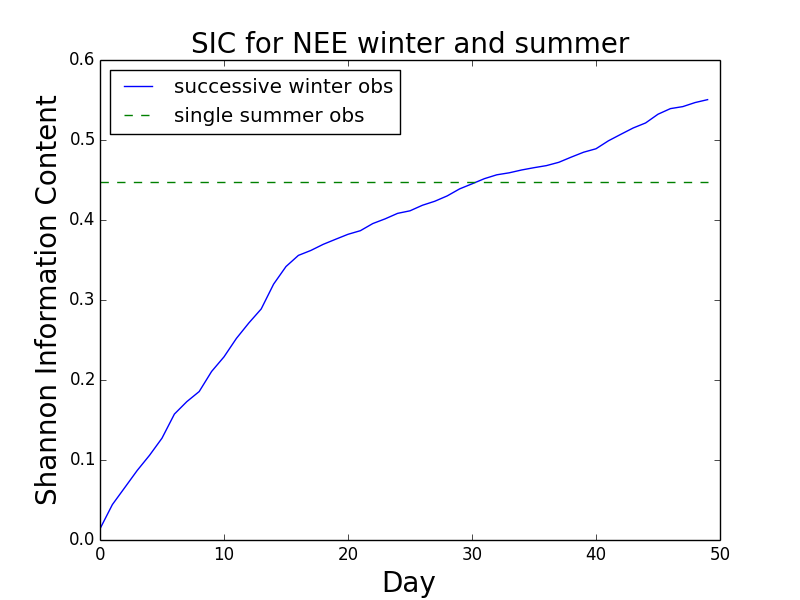
\includegraphics[height=.34\textwidth]{succwinter_singlesummer.png}
\caption{$SIC$ varying as successive observations of $NEE$ are added during winter using driving data from Oregon pine forest. The dashed line shows the $SIC$ for a single observation of $NEE$ made in summer.}
\label{summwintsic}
\end{figure}

Figure \ref{summwintsic} shows us that, for the driver data used in this experiment, we require 31 days of $NEE$ observations to gain the same reduction in entropy for our analysis as 1 observation made in the summer. In the next section (section \ref{DOFS}) we will see that we can reproduce all of the results from sections \ref{sic1time} and \ref{SICsucc} using the degrees of freedom for signal measure of information content. We see that although the $DFS$ correspond to the number of elements of the state measured by the observations and $SIC$ represents the reduction in entropy given a set of observations we still see similar results for both measures.

\section{Degrees of freedom for signal for DALEC} \label{DOFS}%%%%%%%%%%%%%%%%%%%%%%

In this section we repeat some of the experiments from sections \ref{sic1time} and \ref{SICsucc} using the degrees of freedom for signal as a  measure for information content, as described in section \ref{DFSintro}. We use the same $\mathbf{B}$ as in equation \ref{Bmat} and calculate $\mathbf{A}$ by finding and inverting $\mathbf{J}''$ (as in section \ref{sic1time} and \ref{SICsucc}). We begin by plotting the $DFS$ for a single observation of $NEE$ varying with the three years of driving data as in figure \ref{fig:SICNEET} for $SIC$.

\begin{figure}[H]
\centering
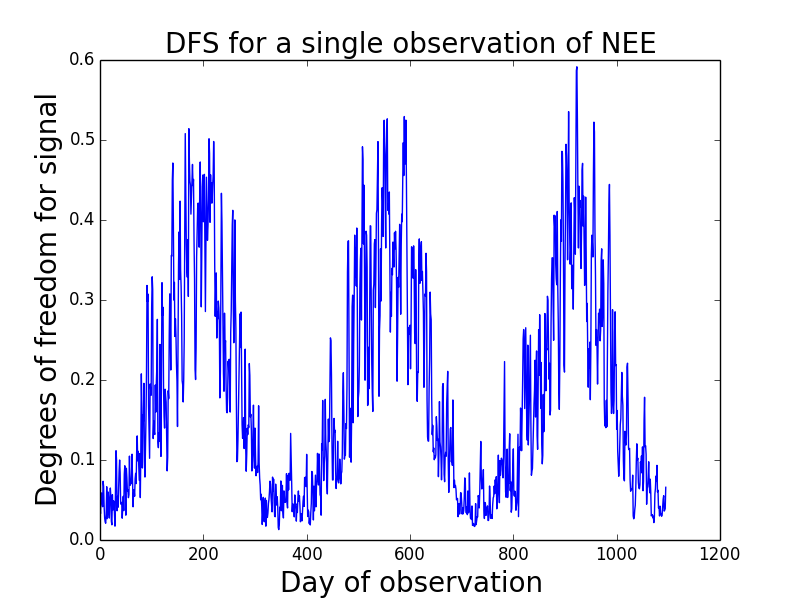
\includegraphics[height=.33\textwidth]{DFS1Obs_0_1095.png}
\caption{$DFS$ varying for a single observation of $NEE$ over three years of driving data from Oregon pine forest.}
\label{DFS1nee}
\end{figure}

We see in figure \ref{DFS1nee} a very similar result as found in figure \ref{fig:SICNEET} with much higher values for the $DFS$ of $NEE$ observations in the summer months, with higher temperatures and higher daily net irradiances. We can repeat the experiment from figure \ref{summwintsic} to show that even when successive observations of $NEE$ are added to our data assimilation window in winter it takes 30 daily winter $NEE$ observations to get the same $DFS$ as 1 observation of $NEE$ made in the summer.

\begin{figure}[H]
\centering
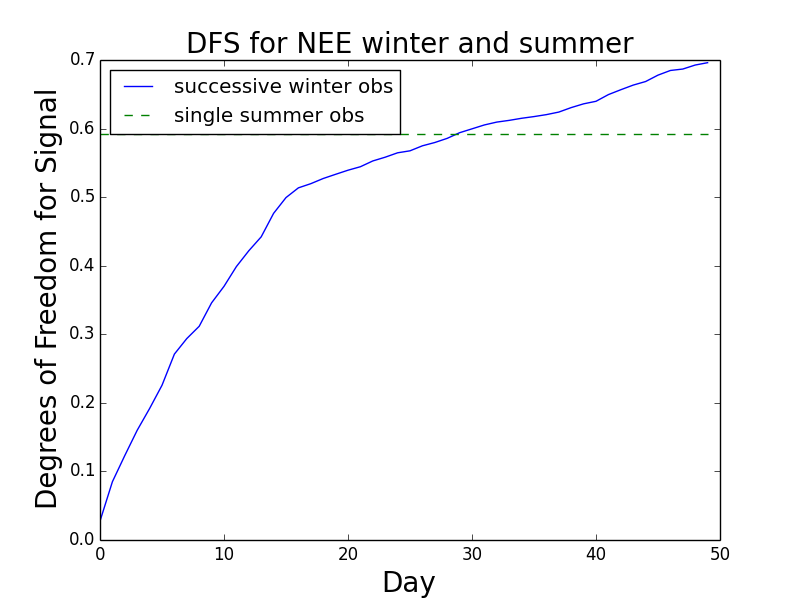
\includegraphics[height=.34\textwidth]{succwinter_singlesummerdofs.png}
\caption{$DFS$ varying as successive observations of $NEE$ are added during winter using driving data from Oregon pine forest. The dashed line shows the $DFS$ for a single observation of $NEE$ made in summer.}
\label{fig:SIC_subplot}
\end{figure}

The value for the $DFS$ corresponds to the number of state elements deemed measured by the observations. Hence when we make a single observation of any of the carbon pools, our $DFS$ value is close to 1 (it is not 1 however as our observations have error) and as successive observations of the same carbon pool are added our $DFS$ value starts tending to 1. However with enough observations over a time window of a single carbon pool we can get a $DFS$ value of greater than 1. This is because the model propagates the state forward in time and we start gaining information about the other connected carbon pools from just observing a single carbon pool. The amount of observations it takes to achieve a $DFS$ of more than 1 corresponds to how dependent the observed carbon pool is on other carbon pools. We can see this effect in figure \ref{dfsobs} where we have plotted the $DFS$ when observing each carbon pool and also $NEE$ for 100 days of observations.

\begin{figure}[H]
\centering
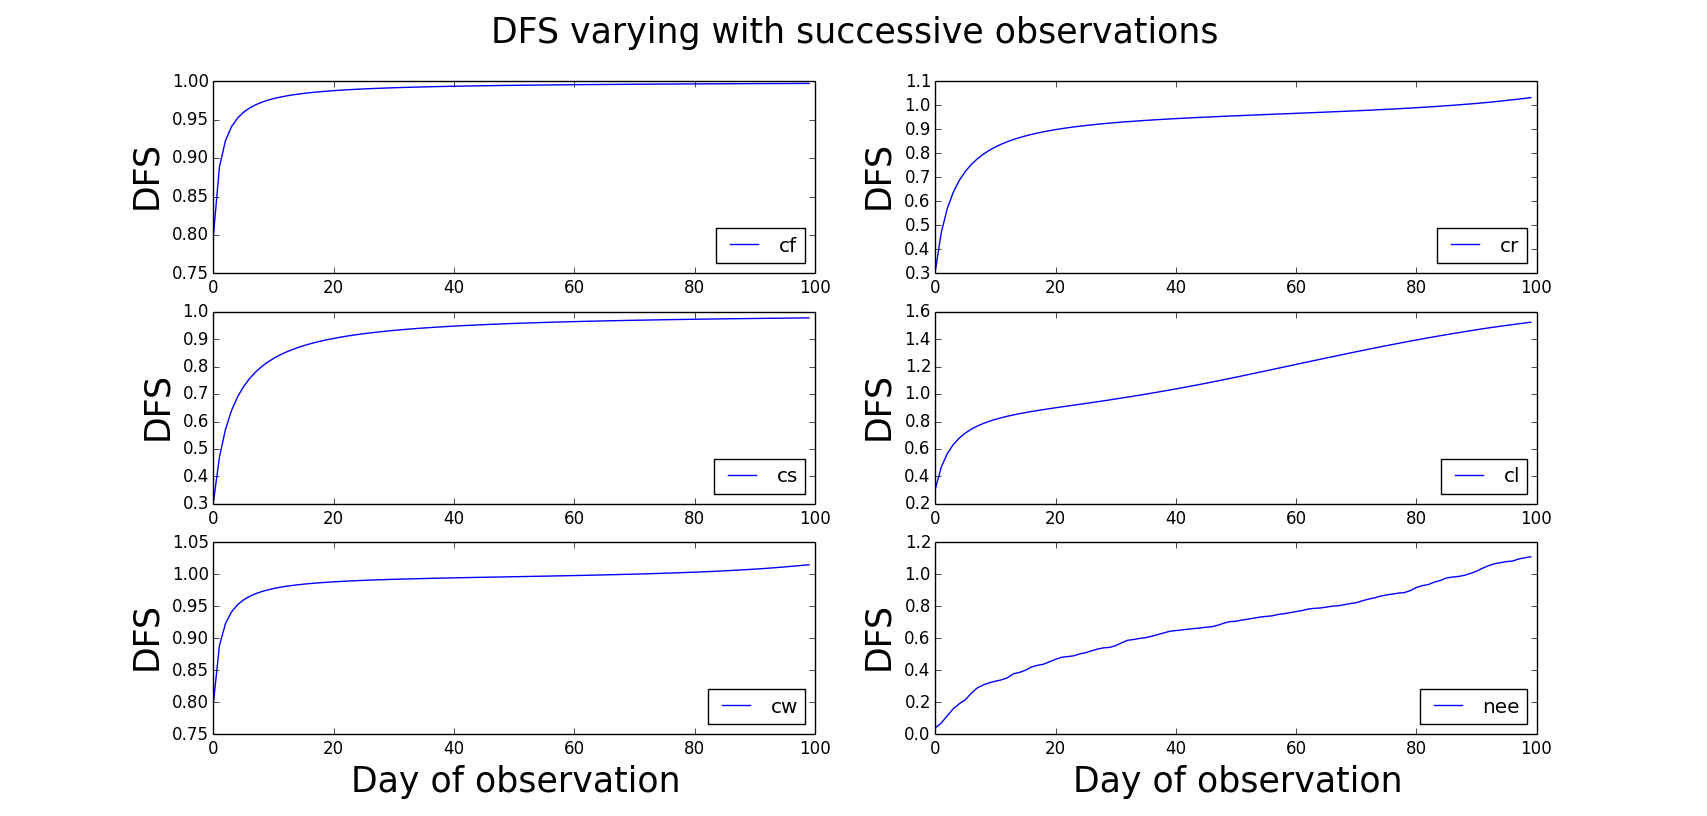
\includegraphics[height=.42\textwidth]{dfssubplt.png}
\caption{$DFS$ varying as successive observations added using 100 days of driving data from Oregon pine forest. Legend in bottom right corner of each plot denotes which observation is being made.}
\label{dfsobs}
\end{figure}

In order to get a higher $DFS$ it is best to observe a variety of different quantities related to different members of the state. We next repeat the experiment from figure \ref{SIC_succ} again for $DFS$ instead of $SIC$.

\begin{figure}[H]
\centering
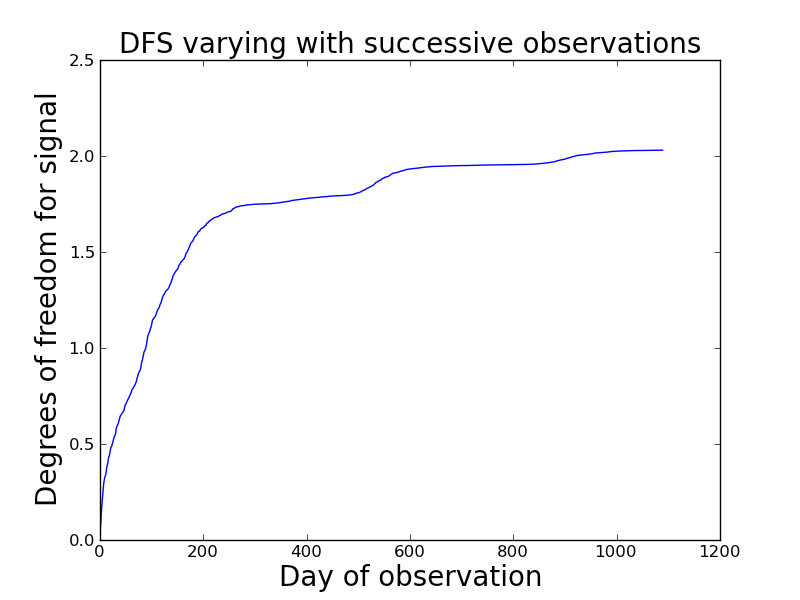
\includegraphics[height=.34\textwidth]{DFS0_1090nee.png}
\caption{$DFS$ varying as successive observations of $NEE$ are added using three years of driving data from Oregon pine forest.}
\label{dfsnee}
\end{figure}

We see a similar result in figure \ref{dfsnee} as in \ref{SIC_succ}. From equation \ref{neeeqn} we see that $NEE$ is a function of 3 of our 5 state elements ($C_f$, $C_l$ and $C_s$), and in figure \ref{dfsnee} it appears that with more observations the $DFS$ may tend to 3. As $NEE$ is not a direct measurement of the carbon pools we do not have our $DFS$ tending to 3 as quickly as an observation of one of the carbon pools tends to 1. 


\section{Conclusion}%%%%%%%%%%%%%%%%%%%%%%

In this report we have taken information content measures previously used in satellite and meteorological data assimilation schemes \cite{stewart2008correlated, fisher2003estimation, sandu2012practical} and applied them to the DALEC carbon balance model \cite{williams2005improved} implemented in a 4D-Var framework. We have looked at the effects of using different observations and different assimilation time windows, using meteorological driving data from a young pine stand in Ponderossa, Oregon for which our version of DALEC is parameterized. 

We have seen that after continually adding the same observation, the information we get from that observation starts to get smaller and eventually we can reduce the entropy of our system no more (or constrain no more elements of our state) with more of the same observation. In order to constrain the most elements of our state (or achieve the maximum possible reduction in entropy for our analysis) it is desirable to take a variety of observations corresponding to different members of the state, if possible. This result is as expected, however, it is important to consider what your state will be when using a forest carbon balance model in a data assimilation framework so that you can identify which observations will correspond to which members of your state and plan your measurement campaign accordingly.

We have also found that $NEE$ observations made in summer are much more valuable than those made in winter, in terms of reducing the entropy of our problem. Although we have used the DALEC carbon balance model for these experiments, $NEE$ is a product of $GPP$ and the respiration fluxes; the $GPP$ function used in DALEC is similar to other such functions from alternative forest carbon balance models, so we would expect to see similar results for these models. $NEE$ observations being more valuable with higher temperatures makes physical sense as this is when $NEE$ observations are of greatest magnitude and give us most information about the fluxes of carbon.    

\bibliography{../PhD}{}
\bibliographystyle{plain}

\section*{Appendix}

\subsection*{The Aggregated Canopy Model}
The aggregated canopy model (ACM) is used in DALEC to calculate $GPP$. The ACM uses the following equations (for more detail please see \cite{williams1997predicting}),
\begin{equation} 
g_c = \frac{|\psi_d|^{a_{10}}}{\frac{1}{2}T_r + a_6 R_{tot}},
\end{equation}
\begin{equation}
p = \frac{a_1NL}{g_c}\text{exp}(T_{max}a_8),
\end{equation}•
\begin{equation}
q = a_3 - a_4,
\end{equation}•
\begin{equation}
C_i = \frac{1}{2}\bigg[C_a + q - p + \sqrt{(C_a + q + p)^{2} - 4(C_aq - pa_3)} \bigg],
\end{equation}•
\begin{equation}
E_0 = \frac{a_7L^2}{L^2 + a_9},
\end{equation}•
\begin{equation}
\delta = -0.408\arccos\bigg(\frac{360(D+10)}{365}\frac{\pi}{180}\bigg),
\end{equation}•
\begin{equation}
s = 24\arccos(-\tan(lat)\tan(\delta))/\pi,
\end{equation}•
\begin{equation}
GPP = \frac{E_0Ig_c(C_a-C_i)}{E_0I + g_c(C_a-C_i)}(a_2s + a_5).
\end{equation}•
The symbols have the following meanings ($a_1,\dots ,a_{10}$ set parameters),
\begin{center}
\begin{tabular}{| l | l |}
\hline
Symbol & Description \\ \hline
$g_c$ & Canopy conductance $(gCm^{-2}day^{-1})$ \\ \hline
$\psi_d$ & Max soil-leaf water potential difference $(MPa)$ \\ \hline
$T_r$ & Daily temperature range $( ^{o}C)$ \\ \hline
$R_{tot}$ & Total plant-soil hydraulic resistance $(MPa m^2s mmol^{-1})$ \\ \hline
$N$ & Foliar nitrogen $(gNm^{-2} \text{ leaf area})$  \\ \hline
$L$ & Leaf area index $(m^2 m^{-2})$ \\ \hline
$T_{max}$ & Maximum daily temperature $( ^{o}C)$  \\ \hline
$C_a$ & Atmospheric $CO_2$ concentration $(\mu mol mol^{-1})$ \\ \hline
$C_i$ & $CO_2$ concentration at site of carboxylation $(\mu mol mol^{-1})$ \\ \hline
$E_0$ & Canopy level quantum yield $(gCMJ^{-1}m^{-2}day^{-1})$ \\ \hline
$\delta$ & Solar declination $(rads)$ \\ \hline
$D$ & Day of year \\ \hline
$s$ & Day length $(hrs)$ \\  \hline  
$lat$ & Site latitude $( ^{o})$ \\ \hline
$I$ & Irradiance $(MJm^{-2}day^{-1})$ \\ 
\hline
\end{tabular}    
\captionof{table}{Symbols used in ACM.}
\end{center}

\subsection*{DALEC rate parameters and initial pool values}

\begin{center}
\begin{tabular}{| l | l | l |}
\hline
Carbon pool & Initial value $(gCm^{-2})$ & Background standard deviation (as a \% of initial pool) \\ \hline
$C_f$ & 58 & 20\% \\ \hline
$C_r$ & 102 & 20\% \\ \hline
$C_w$ & 770 & 20\% \\ \hline
$C_l$ & 40 & 20\% \\ \hline
$C_s$ & 9897 & 20\% \\ 
\hline
\end{tabular}    
\captionof{table}{Inital carbon pool values for the DALEC model and the standard deviations expressed as a percentage of the initial value. }
\end{center}

\begin{center}
\begin{tabular}{| l | l | l |}
\hline
Parameter & Description & Value \\ \hline
$p_1 $ & decomposition rate & $4.41\times 10^{-6}$ \\ \hline
$p_2 $ & fraction of $GPP$ respired & $0.47$ \\ \hline
$p_3 $ & fraction of $GPP$ allocated to foliage & $0.31$ \\ \hline
$p_4 $ & fraction of $GPP$ allocated to roots & $0.43$ \\ \hline
$p_5 $ & turnover rate of foliage & $2.7\times 10^{-3}$ \\ \hline
$p_6 $ & turnover rate of woods & $2.06\times 10^{-6}$ \\ \hline
$p_7 $ & turnover rate of roots & $2.48\times 10^{-3}$ \\ \hline
$p_8 $ & mineralisation rate of $C_l$ & $2.28\times 10^{-2}$ \\ \hline
$p_9 $ & mineralisation rate of $C_s$ & $2.65\times 10^{-6}$ \\ 
\hline
\end{tabular}    
\captionof{table}{Parameters for evergreen DALEC.}
\end{center}



\end{document}